\documentclass[12pt,letterpaper]{article}

\usepackage{amsfonts}
\usepackage{graphics}
\usepackage{graphicx}
\usepackage{colortbl}
\usepackage{amsmath}

\usepackage{algorithm}
\usepackage[noend]{algpseudocode}
\usepackage{array}

\usepackage{epstopdf}

\setlength\intextsep{10pt}
\setlength\textfloatsep{10pt}

\newenvironment{proof}{\noindent{\bf Proof:}}{\qed\bigskip}

\newtheorem{theorem}{Theorem}
\newtheorem{corollary}{Corollary}
\newtheorem{lemma}{Lemma} 
\newtheorem{claim}{Claim}
\newtheorem{fact}{Fact}
\newtheorem{definition}{Definition}
\newtheorem{assumption}{Assumption}
\newtheorem{observation}{Observation}
\newtheorem{example}{Example}
\newcommand{\qed}{\rule{7pt}{7pt}}

\newcommand{\assignment}[4]{
\thispagestyle{plain} 
\newpage
\setcounter{page}{1}
\noindent
\begin{center}
\framebox{ \vbox{ \hbox to 6.28in
{\bf CS578/STAT590: Introduction Machine Learning \hfill #1}
\vspace{4mm}
\hbox to 6.28in
{\hspace{2.5in}\large\mbox{Problem Set #2}}
\vspace{4mm}
\hbox to 6.28in
{{\it Handed Out: #3 \hfill Due: #4}}
}}
\end{center}
}

\newcommand{\solution}[4]{
\thispagestyle{plain} 
\newpage
\setcounter{page}{1}
\noindent
\begin{center}
\framebox{ \vbox{ \hbox to 6.28in
{\bf CS578/STAT590: Introduction to Machine Learning \hfill #4}
\vspace{4mm}
\hbox to 6.28in
{\hspace{2.5in}\large\mbox{Problem Set #3}}
\vspace{4mm}
\hbox to 6.28in
{#1 \hfill {\it Handed In: #2}}
}}
\end{center}
\markright{#1}
}



\def\Comment#1{\textsf{\textsl{$\langle\!\langle$#1\/$\rangle\!\rangle$}}}



\oddsidemargin 0in
\evensidemargin 0in
\textwidth 6.5in
\topmargin -0.5in
\textheight 9.0in

\begin{document}

\solution{Gen Nishida}{\today}{4}{Fall 2014}
% Fill in the above, for example, as follows:
% \solution{John Smith}{\today}{1}{Fall 2014}

\pagestyle{myheadings}  % Leave this command alone

\section*{Questions}

\begin{enumerate}
\item {\bf Boosting}

\begin{enumerate}
\item[(1)] The weak hypothesis used at each round, and its error

{\bf 1st round} $h_1(x)={\rm sign} (x_1>6)$, $\epsilon_1=0.2$ ($\alpha_1=0.6931$)

\begin{table}[htb]
  \begin{center}
  \begin{tabular}{|c|c|c|c|c|} \hline
    index & $x_1$ & $x_2$ & $y$ & prediction \\ \hline
    1 & 1 & 10 & - & - \\ \hline
    2 & 4 & 4 & - & -\\ \hline
    3 & 8 & 7 & + & + \\ \hline
    4 & 5 & 6 & - & - \\ \hline
    5 & 3 & 16 & - & - \\ \hline
    6 & 7 & 7 & + & + \\ \hline
    7 & 10 & 14 & + & + \\ \hline
    8 & 4 & 2 & - & - \\ \hline
    9 & 4 & 10 & + & - \\ \hline
    10 & 8 & 8 & - & + \\ \hline
  \end{tabular}
  \caption{The prediction by $h_1$}
  \label{tab:1st_round_prediction}
  \end{center}
\end{table}

{\bf 2nd round} $h_2(x)=sign (x_2>9)$, $\epsilon_1=0.25$ ($\alpha_2=0.5493$)

\begin{table}[htb]
  \begin{center}
  \begin{tabular}{|c|c|c|c|c|} \hline
    index & $x_1$ & $x_2$ & $y$ & prediction \\ \hline
    1 & 1 & 10 & - & + \\ \hline
    2 & 4 & 4 & - & - \\ \hline
    3 & 8 & 7 & + & - \\ \hline
    4 & 5 & 6 & - & - \\ \hline
    5 & 3 & 16 & - & + \\ \hline
    6 & 7 & 7 & + & - \\ \hline
    7 & 10 & 14 & + & + \\ \hline
    8 & 4 & 2 & - & - \\ \hline
    9 & 4 & 10 & + & + \\ \hline
    10 & 8 & 8 & - & - \\ \hline
  \end{tabular}
  \caption{The prediction by $h_1$}
  \label{tab:1st_round_prediction}
  \end{center}
\end{table}

\item[(2)] The distribution $D_i$ over the examples for each round

The distribution $D_i$ evolves over the rounds as shown in Table \ref{tab:distribution_evolution}.

\begin{table}[htb]
  \begin{center}
  \begin{tabular}{|c|c|c|c|c|} \hline
    index & $D_1$ & $D_2$ & $D_3$ \\ \hline
    1 & 0.1 & 0.0625 & 0.125 \\ \hline
    2 & 0.1 & 0.0625 & 0.0417 \\ \hline
    3 & 0.1 & 0.0625 & 0.125 \\ \hline
    4 & 0.1 & 0.0625 & 0.0417 \\ \hline
    5 & 0.1 & 0.0625 & 0.125 \\ \hline
    6 & 0.1 & 0.0625 & 0.125 \\ \hline
    7 & 0.1 & 0.0625 & 0.0417 \\ \hline
    8 & 0.1 & 0.0625 & 0.0417 \\ \hline
    9 & 0.1 & 0.25 & 0.1666 \\ \hline
    10 & 0.1 & 0.25 & 0.1666 \\ \hline
  \end{tabular}
  \caption{The distribution $D_i$}
  \label{tab:distribution_evolution}
  \end{center}
\end{table}

\item[(3)] The final hypothesis after running two rounds.

$H_{\rm final}(x)={\rm sign} \left[ 0.6931 \times {\rm sign}(x_1 > 6) + 0.5493 \times {\rm sign}(x_2 > 9) \right]$

\end{enumerate}

\item {\bf Naive Bayes}

\begin{enumerate}
\item[(1)] Write the joint log-likelihood of a document and labels (i.e., $\log P(D_i, y_i)$).

First, the joint probability $P(D_i, y_i)$ is
\[
\left[ \frac{n!}{a_i!b_i!c_i!d_i!}\alpha_1^{a_i}\beta_1^{b_i}\gamma_1^{c_i}\delta_1^{d_i} \times P(y_i=1)\right]^{y_i} \times \left[ \frac{n!}{a_i!b_i!c_i!d_i!}\alpha_0^{a_i}\beta_0^{b_i}\gamma_0^{c_i}\delta_0^{d_i} \times P(y_i=0)\right]^{(1-y_i)}
\]
Since we do not know a prior probability of $P(y)$, we just use the uniform distribution, which is $P(y)=1/2$. Thus,
\[
\frac{1}{2} \times \left[ \frac{n!}{a_i!b_i!c_i!d_i!}\alpha_1^{a_i}\beta_1^{b_i}\gamma_1^{c_i}\delta_1^{d_i}\right]^{y_i} \times \left[ \frac{n!}{a_i!b_i!c_i!d_i!}\alpha_0^{a_i}\beta_0^{b_i}\gamma_0^{c_i}\delta_0^{d_i}\right]^{(1-y_i)}
\]
Then, its logarithm becomes
\begin{eqnarray}
\log \frac{1}{2} + y_i \log \left[ \frac{n!}{a_i!b_i!c_i!d_i!}\alpha_1^{a_i}\beta_1^{b_i}\gamma_1^{c_i}\delta_1^{d_i}\right] + (1-y_i) \log \left[ \frac{n!}{a_i!b_i!c_i!d_i!}\alpha_0^{a_i}\beta_0^{b_i}\gamma_0^{c_i}\delta_0^{d_i}\right]
 \nonumber \\
= \log \frac{1}{2} + \log \frac{n!}{a_i!b_i!c_i!d_i!} + y_i \left[ a_i \log \alpha_1 + b_i \log \beta_1 + c_i \log \gamma_1 + d_i \log \delta_1 \right] \nonumber \\ + (1-y_i) \left[ a_i \log \alpha_0 + b_i \log \beta_0 + c_i \log \gamma_0 + d_i \log \delta_0 \right] \nonumber
\end{eqnarray}

\end{enumerate}

\item {\bf Bayesian Network}
\begin{enumerate}

\item[(1)] How many parameters are needed to define the network?

{\bf 21 parameters}

A requires 1 parameter, and B requires 2 parameters. For C, there are $2 \times 3 = 6$ combinations of A and B and for each A and B, it requires 2 parameters, so $6 \times 2 = 12$ parameters. Finally, D requires $3 \times 2 = 6$ parameters. Thus, 1 + 2 + 12 + 6 = 21 parameters are required in total.

\item[(2)] Write the expression calculating 

(a) $P(A=1, D=2)$ 

\begin{eqnarray}
& = & \sum_{B,C} P(A=1,B,C,D=2) \nonumber \\
& = & \sum_{B,C} P(A=1)P(B)P(C|A=1,B)P(D=2|C) \nonumber
\end{eqnarray}

(b) $P(A=1,D=2|C=1)$

\begin{eqnarray}
& = & \frac{\sum_B P(A=1,B,C=1,D=2)}{P(C=1)} \nonumber \\
& = & \frac{\sum_B P(A=1)P(B)P(C=1|A=1,B)P(D=2|C=1)}{P(C=1)} \nonumber
\end{eqnarray}

\end{enumerate}

\item {\bf Variable Elimination}

\begin{enumerate}

\item[(1)] Write the expression calculating P(Marry calls), according to the network below. How many operations are needed to compute it?

{\bf 79 operations in total}.

\[
\sum_{E,B,A,J} P(E)P(B)P(A|B,E)P(J|A)P(M|A)
\]

The product consists of 5 terms, which requires 4 multiplications. Also, since each summation with regard to $E$, $B$, $A$, and $J$ requires two iterations, the number of multiplications becomes $4 \times 2^4 = 64$ in addition to $2^4-1=15$ additions. Thus, $64+15=79$ operations are required in total.

\item[(2)] Run the variable elimination algorithm. How many operations are needed now? (Write down each step)

{\bf 23 operations in total}.

At each step, we eliminate a variable which has the fewst degree in the interaction graph (Figure \ref{fig:interaction_graph}).

1) Eliminate J

\[
=\sum_{E,B,A} P(E)P(B)P(A|B,E)P(M|A)f_1(A)
\]
where $f_1 (A)=\sum_J P(J|A)$. Apparently, $f_1 (A)=1$, so no operation is required for this elimination.

2) Eliminate E

\[
=\sum_{B,A} P(B)P(M|A) f_1 (A) f_2 (A,B)
\]
where $f_2 (A,B)=\sum_E P(E)P(A|B,E)$. For each pair of $A$ and $B$, one multiplication is required for each $E$, so the number of multiplications is 2. Also, the summation requires 1 addition. Therefore, 3 operations are necessary for each pair of $A$ and $B$. Since we have $2^2=4$ combinations of $A$ and $B$, $3 \times 4 = 12$ operations are required for $f_2 (A,B)$.

3) Eliminate B

\[
=\sum_{A} P(M|A) f_1 (A) f_3 (A)
\]
where $f_3 (A)=\sum_B P(B)f_2 (A,B)$. For a given $A$, one addition and two multiplications are necessary. Thus, $3 \times 2 = 6$ operations are required for $f_3 (A)$.

4) Eliminate A
\[
f_4 (M)=\sum_{A} P(M|A) f_1 (A) f_3 (A)
\]
We need two multiplications for each $A$, so $2 \times 2 = 4$ multiplications are required. Also, we need one addition for summation. Thus, $4 + 1 = 5$ operations are requried for $f_4 (M)$. To sumarize, we need $12 + 6 + 5 = 23$ operations are required in total. Note that the number of operations are much less than the one without variable elimination.

\begin{figure}[hbtp]
\centering
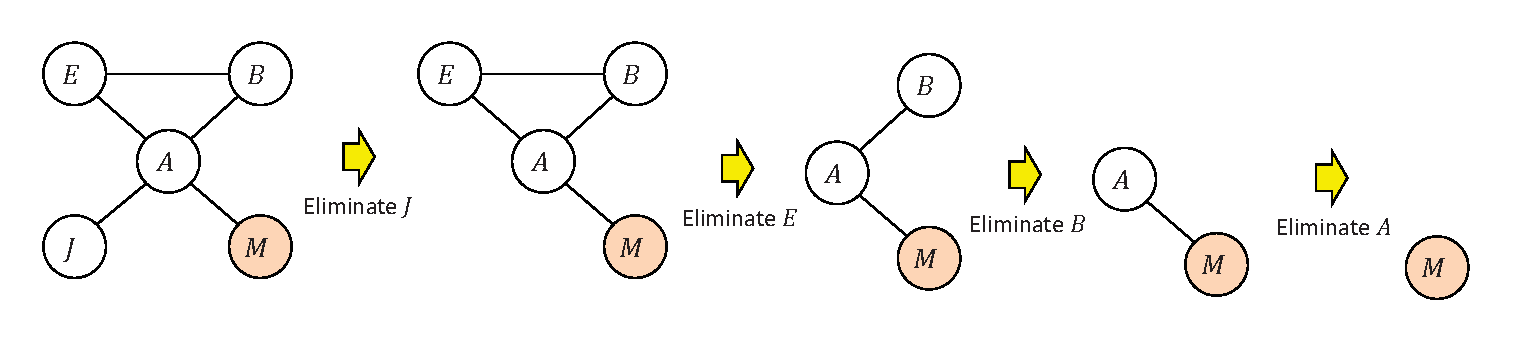
\includegraphics[width=160mm]{interaction_graph}
\caption{This figure shows how the interaction graph changes over the variable eliminations. Note that at each step the node which has the fewest degrees in the graph is chosen to eliminate.}
\label{fig:interaction_graph}
\end{figure}

\end{enumerate}


\end{enumerate}

\end{document}

